%!TEX root = ../Thesis.tex
%\chapter{Long chapter title with $\pi$ $π$ or π}
%\chapter{Long chapter title with \texorpdfstring{$\pi$ $π$ or π}{π π or π}}
\section[Deep Learning Application for 4D Pressure Saturation Inversion Compared to Bayesian Inversion on North Sea Data]{Deep Learning Application\\for 4D Pressure Saturation Inversion Compared to Bayesian Inversion on\\North Sea Data}

\paragraph{Abstract:} In this work we present a deep neural network inversion on map-based 4D seismic data for pressure and saturation. We present a novel neural network architecture that trains on synthetic data and provides insights into observed field seismic. The network explicitly includes AVO gradient calculation within the network as physical knowledge to stabilize pressure and saturation changes separation. We apply the method to Schiehallion field data and go on to compare the results to Bayesian inversion results. Despite not using convolutional neural networks for spatial information, we produce maps with good signal to noise ratio and coherency.

\subsection*{Key points:}
\begin{itemize}
    \item Physics-based \acl{dnn}
    \item AVO gradient calculation in network architecture stabilizes prediction
    \item Variational bottleneck to buffer noisy inputs
    \item Noise injection at input to transfer from simulation to field data
\end{itemize}

{\vfill\hfill\newline\fbox{\parbox{.97\textwidth}{\fullcite{dramsch2019deep}}}}

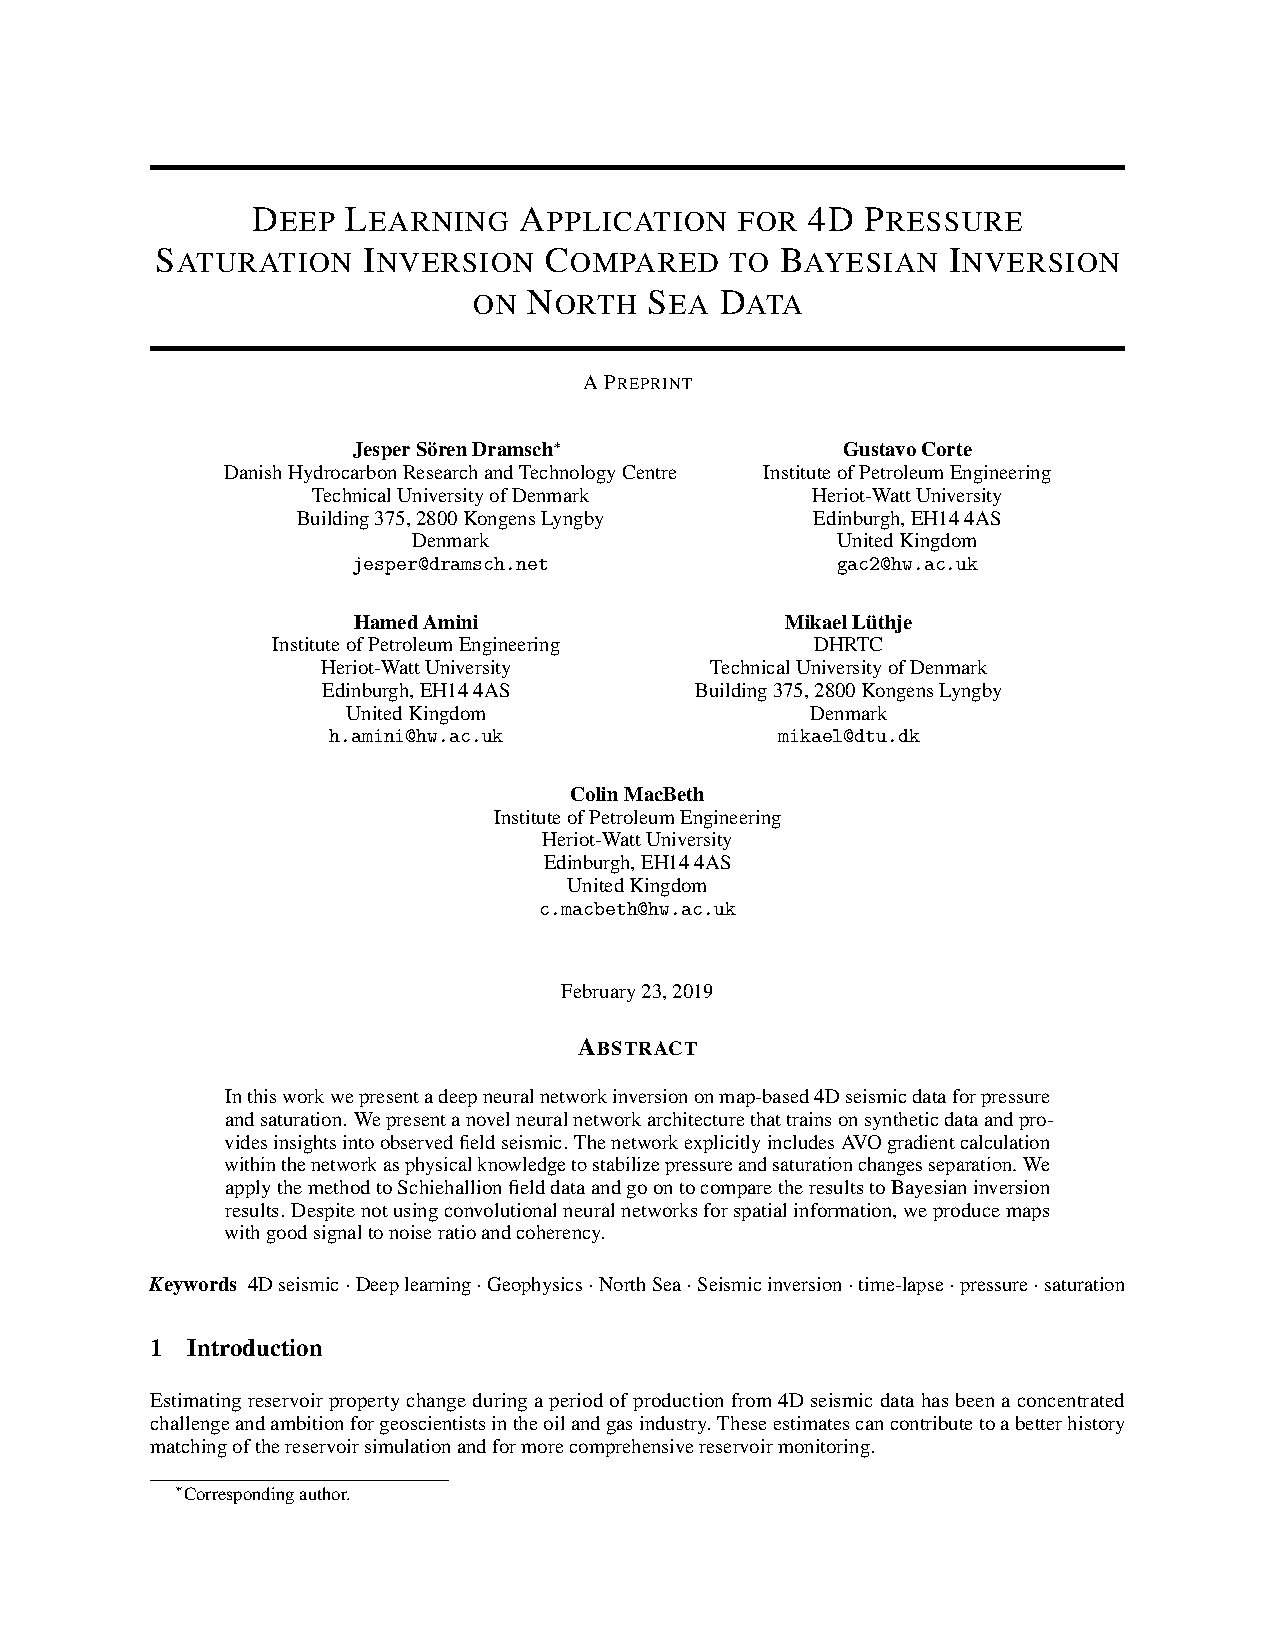
\includepdf[pages={1-6},pagecommand={},width=1.2\textwidth,offset=0.7cm -1.5cm]{papers/2019.2}
